\id{МРНТИ 06.52.13}{}

\begin{articleheader}
\sectionwithauthors{Ж.C.Булхаирова, А.Е. Шоман, А.К.Байдаков}{ИНТЕГРИРОВАННЫЕ СИСТЕМЫ ВЕРТИКАЛЬНОГО ФЕРМЕРСТВА, НАЦЕЛЕННЫЕ НА УСТОЙЧИВОЕ ПРОИЗВОДСТВО СЕЛЬСКОХОЗЯЙСТВЕННОЙ ПРОДУКЦИИ В ГОРОДСКОЙ СРЕДЕ}

{\bfseries
\textsuperscript{1}Ж.C.Булхаирова\textsuperscript{\envelope },
\textsuperscript{1}А.Е. Шоман,
\textsuperscript{2}А.К.Байдаков
}
\end{articleheader}

\begin{affiliation}
\textsuperscript{1}ТОО «Astana IT University», г. Астана, Казахстан,

\textsuperscript{2}Казахский агротехнический исследовательский университет им. С.Сейфуллина, Астана, Казахстан

\raggedright \textsuperscript{\envelope }Корреспондент-автор: honeyzhu@mail.ru
\end{affiliation}

В статье рассмотрены вопросы интегрированной системы вертикального
фермерства, нацеленные на устойчивое производство сельскохозяйственной
продукции в городской среде. Основная концепция вертикального фермерства
заключается в том, что оно нацелено на устойчивое развитие сельского
хозяйства, обеспечение населения продовольственной безопасностью,
использованием новых технологий в условиях городской среды.
Интегрированные системы вертикального фермерства дает возможность
фермерам получить более высокий урожай и при этом меньше затрачивая на
его производство, особенно значительно уменьшаются логистические затраты
по сравнению с традиционным сельским хозяйством. В ходе проведения
данного исследования авторами проводился обзор зарубежного опыта
развития вертикального фермерства в таких странах как: США, Китай,
Сингапур, Япония. Также представлены и проанализированы статистические
данные по текущему состоянию и доля рынка вертикального фермерства в
мире. Авторами была также проанализирован рынок вертикального фермерства
в Казахстане и приведены примеры действующих вертикальных ферм в стране.
Стоит отметить, что наиболее перспективным развитием рынка вертикальных
ферм в Казахстане становится в области выращивания микрозелени,
приведены преимущества развития интегрированных систем вертикального
фермерства в городской среде по сравнению с традиционным. Авторами была
определена и представлены данные по урожайности вертикальной фермы по
сравнению с традиционным сельским хозяйством. Необходимо отметить, что в
рамках осуществляемого проекта были разработаны и изготовлена
специализированная экспериментальная гидропонная установка для
проведения исследований по выращиванию рассады томата и листового
салата. Стоит отметить, что интегрированные системы вертикального
фермерства, нацеленные на устойчивое производство сельскохозяйственной
продукции в городской среде -- продовольственная безопасность и
сохранение качества продукции -- пищевая безопасность.

{\bfseries Ключевые слова:} интегрированные системы, вертикальные
фермерства, устойчивое производство, сельскохозяйственная, продукция,
городская среда.

\begin{articleheader}
{\bfseries ҚАЛАЛЫҚ ОРТАДА АУЫЛШАРУАШЫЛЫҚ ӨНІМДЕРІН ТҰРАҚТЫ ӨНДІРУГЕ БАҒЫТТАЛҒАН ИНТЕГРАЦИЯЛАНҒАН ТІК ЕГІНШІЛІК ЖҮЙЕЛЕРІ}

{\bfseries
\textsuperscript{1}Ж.С.Булхаирова\textsuperscript{\envelope },
\textsuperscript{1}А.Е. Шоман,
\textsuperscript{2}А.К.Байдаков
}
\end{articleheader}

\begin{affiliation}
\textsuperscript{1}«Astana IT University» ЖШС, Астана, Қазақстан,

\textsuperscript{2}С.Сейфуллин атындағы Қазақ агротехникалық зерттеу университеті, Астана, Қазақстан,

e-mail: honeyzhu@mail.ru
\end{affiliation}

Мақалада қалалық ортада ауыл шаруашылығы өнімдерін тұрақты өндіруге
бағытталған интеграцияланған тік егіншілік жүйесінің мәселелері
қарастырылады. Тік фермерліктің негізгі тұжырымда\-масы-бұл ауыл
шаруашылығын тұрақты дамытуға, халықты азық-түлік қауіпсіздігімен
қамтамасыз етуге, қалалық ортада жаңа технологияларды қолдануға
бағытталған. Интеграцияланған тік егіншілік жүйелері фермерлерге жоғары
өнім алуға мүмкіндік береді және оны өндіруге аз жұмсайды, әсіресе
дәстүрлі ауыл шаруашылығымен салыстырғанда логистикалық шығындар
айтарлықтай төмендейді. Осы зерттеуді жүргізу барысында авторлар АҚШ,
Қытай, Сингапур, Жапония сияқты елдерде тік фермерлікті дамытудың
шетелдік тәжірибесіне шолу жасады. Сондай-ақ, қазіргі жағдай бойынша
статистика және әлемдегі тік фермерлік нарықтың үлесі ұсынылып,
талданды. Сондай-ақ, авторлар Қазақстандағы тік фермерлік нарығын
талдап, елдегі жұмыс істеп тұрған тік фермалардың мысалдарын келтірді.
Айта кету керек, Қазақстандағы тік фермалар нарығының неғұрлым
перспективалы дамуы микрожасылдарды өсіру саласында болып отыр, дәстүрлі
фермамен салыстырғанда қалалық ортада тік фермерліктің интеграцияланған
жүйелерін дамытудың артықшылықтары келтірілген. Авторлар дәстүрлі ауыл
шаруашылығымен салыстырғанда тік ферманың өнімділігі туралы деректерді
анықтады және ұсынды. Айта кету керек, жүзеге асырылып жатқан жоба
аясында қызанақ пен жапырақ салатының көшеттерін өсіру бойынша
зерттеулер жүргізу үшін мамандандырылған эксперименттік гидропоникалық
қондырғы жасалды және жасалды. Айта кету керек, қалалық ортада ауыл
шаруашылығы өнімдерін тұрақты өндіруге бағытталған интеграцияланған тік
фермерлік жүйелер -- азық -- түлік қауіпсіздігі және өнім сапасын
сақтау-азық-түлік қауіпсіздігі.

{\bfseries Түйін сөздер:} интеграцияланған жүйелер, тік егіншілік, тұрақты
өндіріс, ауылшаруашылық, \\өнімдері, қалалық орта.

\begin{articleheader}
{\bfseries INTEGRATED VERTICAL FARMING SYSTEMS BASED ON SUSTAINABLE AGRICULTURAL PRODUCTION IN AN URBAN ENVIRONMENT}

{\bfseries
\textsuperscript{1}Zh.S. Bulkhairova\textsuperscript{\envelope },
\textsuperscript{1}A.E. Shoman,
\textsuperscript{2}A.K. Baidakov
}
\end{articleheader}

\begin{affiliation}
\textsuperscript{1}«Astana IT University» LLC, Astana, Kazakhstan,

\textsuperscript{2}S.Seifullin Kazakh Agrotechnical Research University, Astana, Kazakhstan,

e-mail: honeyzhu@mail.ru
\end{affiliation}

The article discusses the issues of an integrated vertical farming
system aimed at sustainable agricultural production in an urban
environment. The main concept of vertical farming is that it is aimed at
sustainable agricultural development, providing the population with food
security, using new technologies in an urban environment. Integrated
vertical farming systems enable farmers to obtain a higher yield and at
the same time spend less on its production, especially significantly
reducing logistical costs compared to traditional agriculture. In the
course of this study, the authors conducted a review of foreign
experience in the develop\-ment of vertical farming in such countries as
the USA, China, Singapore, Japan. Statistical data on the current state
and market share of vertical farming in the world are also presented and
analyzed. The authors also analyzed the vertical farming market in
Kazakhstan and gave examples of operating vertical farms in the country.
It is worth noting that the most promising development of the vertical
farm market in Kazakhstan is in the field of micro-greenery cultivation,
the advantages of developing integrated vertical farming systems in an
urban environment compared to traditional ones are given. The authors
determined and presented data on the yield of a vertical farm compared
to traditional agriculture. It should be noted that within the framework
of the ongoing project, a specialized experimental hydroponic
installation was developed and manufactured to conduct research on
growing tomato seedlings and lettuce. It is worth noting that integrated
vertical farming systems aimed at sustainable agricultural production in
an urban environment -- food safety and preservation of product quality
-- food safety.

{\bfseries Keywords:} integrated systems, vertical farming, sustainable
production, agricultural, products, urban environment.

\begin{multicols}{2}
{\bfseries Введение.} При современном уровне развития мира численность
населения стремительно растет, что требует увеличения объемов
сельскохозяйственного производства. Следовательно, поиск нетрадиционных
методов ведения сельского хозяйства, то есть устойчивых интегрированных
сельскохозяйственных систем, направленных на создание
сельскохозяйственной продукции в городах, представляет собой эффективное
решение проблем производства продовольствия. Вертикальные фермерские
системы - это сельскохозяйственная концепция, направленная на устойчивое
производство сельскохозяйственной продукции в городах и обеспечение
населения продовольствием за счет применения современных технологий и
креативных решений по использованию вертикальных пространств {[}1{]}. В
отличие от традиционного сельского хозяйства, в городах, где в будущем
будет проживать две трети населения планеты, необходимо применять
сложные методы ведения сельского хозяйства. Интегрированные системы
вертикального фермерства позволяют получать хорошие урожаи с небольшой
площади и контролировать практически все аспекты: орошение, температуру,
воздух, свет, качество воды и питание.

Основной целью статьи является раскрытие преимущества развития
интегрированных систем вертикального фермерства, нацеленные на
устойчивое производство сельскохозяйственной продукции в городской
среде, в Казахстане. Исходя из поставленной цели были поставлены
следующие задачи: проанализировать международный опыт развития
вертикального фермерства, проанализировать мировую долю рынка
вертикального фермерство и показать преимущества применения
интегрированных систем вертикального фермерства в городской среде
Казахстана.

Необходимо отметить, что концепция вертикального фермерства существует
уже несколько десятилетий, но она по-прежнему важна и необходима.
Интегрированные системы вертикального фермерства также положительно
влияют на окружающую среду, поскольку потребляют меньше энергии,
производят меньше загрязняющих веществ и не требуют использования
тяжелой техники, пестицидов и удобрений. Выращивание
сельскохозяйственной продукции в городской среде с использованием
передовых сельскохозяйственных технологий дает реальный контроль над
необходимыми растениям ресурсами, делая их рост и развитие
предсказуемыми и управляемыми. Сама технология - интегрированная система
вертикального фермерства - может решить проблему обеспечения растущего
городского населения достаточным количеством продовольствия.
Интегрированные системы вертикального фермерства в городах часто
используют методы беспочвенного земледелия, такие как аквапоника,
гидропоника и аэропоника, которые требуют лишь десять процентов воды по
сравнению с традиционными фермами сельского хозяйства. Данные технологии
позволяют перерабатывать и/или реализовывать сельскохозяйственную
продукцию независимо от климатических условий региона, в котором
находится ферма, и позволяют производить новые продукты без
использования пестицидов и гербицидов. Что еще более важно, вертикальные
фермы снижают сельскохозяйственные затраты по сравнению с традиционным
сельским хозяйством за счет сокращения расстояния между производителем и
потребителем - логистических издержек {[}2{]}. Важно отметить, что,
несмотря на растущую популярность органического земледелия,
интегрированные системы вертикального фермерства по выращиванию
сельскохозяйственной продукции в городах привели к развитию бизнеса «под
ключ», или, другими словами, «софта» для ферм.

{\bfseries Материалы и методы.} Исследование выполнено при финансовой
поддержке Комитета науки Министерства науки и высшего образования
Республики Казахстан в рамках ПЦФ ИРН: BR24992852 на тему «Разработка
интеллектуальных моделей и методов цифровой экосистемы Smart City для
устойчивого развития города и повышения качества уровни жизни горожан».

Для написания статьи авторы использовали следующие методы:

- Аналитико-обзорная оценка, который был представлен в виде
систематического обзора зарубежного опыта по вертикальному фермерству
(например такие страны, как США, Китай, Сингапур, Япония), анализа
научной литературы и статей в области устойчивых агротехнологий в
городской среде, сбор и анализ статистических данных о текущем состоянии
мирового и казахстанского рынков вертикального фермерства и
идентификация актуальных вызовов таких как рост численности населения,
уменьшение пахотных земель, климатические вызовы, дефицит ресурсов
(проблема с водными ресурсами, деградация земель, возобновляемая энергия
и т.д.).

- Эмпирическая и сравнительно-эксперимент\-альная оценка, в которой
применялись эмпирические методы такие как: сравнительный анализ
урожайности вертикального и традиционного сельского хозяйства, оценка
ресурсной эффективности, выбор наиболее перспективных культур для
городской среды таких как: свекла, эстрагон.

- Оценка экономической эффективности вертикального фермерства
посредством анализа рентабельности интегрированных систем вертикального
фермерства в условиях городской среды (например, уменьшение
логистических и производственных затрат, прогноз роста рынка
вертикального фермерства в мире и Казахстане.

Таким образом, методология исследования данного исследования была
построена на комплексном подходе: от теоретического анализа глобальных и
локальных трендов в вертикальном фермерстве до практической реализации
экспериментальной установки и оценки ее эффективности. Это позволило
авторам предложить научно обоснованные рекомендации и продемонстрировать
реальные преимущества внедрения интегрированных систем вертикального
фермерства в условиях городской среды.

{\bfseries Результаты и обсуждение.} Интегрированные системы вертикального
фермерства - новый и популярный вид сельского хозяйства, который часто
используется в местах, где традиционное земледелие невозможно или
невыгодно. Идея интегрированных систем «вертикального земледелия
возникла уже давно. Сегодня вертикальная ферма располагается в хорошо
спланированном высотном здании или в соответствующим образом
переоборудованном промышленном здании, реже - в административном здании,
расположенном в городе или рядом с ним, с системами выработки
электроэнергии, отопления и охлаждения, переработки и утилизации отходов
и так далее. Одним словом, вертикальная ферма - это высокотехнологичная
теплица, в которой растения получают достаточное количество света и
естественного освещения благодаря высокой влажности и температурному
режиму, обеспечиваемому одноламповыми светодиодными фитолампами,
гидропонной или аэропонной технологией и кондиционированием воздуха
{[}3{]}.

Технология вертикального фермерства была разработана около десяти лет
назад и уже активно используется в таких странах как: Америка, Канада,
Швеция, Япония и других развитых странах северного полушария, а также в
Австралии, где есть обширные пустынные территории {[}3{]}. Впервые
вертикальные фермы были построены в 2012 году. Сингапур и Япония
считаются первыми странами, создавшими интегрированные
сельскохозяйственные системы вертикального фермерства, поскольку они
имеют большое население и небольшие земельные площади {[}4{]}. Япония
была одной из первых стран, внедривших и разработавших концепцию
интегрированные системы вертикального фермерства в городских районах.
Одним из успешных примеров вертикального фермерства является компания
«Mirai Shokuhin», которая в 2004 году открыла свою первую вертикальную
ферму в Камакуре, который находится в пятидесяти километрах к юго-западу
от Токио. Первоначально на ферме выращивали различные виды
салата-латука. Стоит отметить, что благодаря гидропонной системе и
светодиодному освещению создаются оптимальные условия для успешного
роста растений. «Mirai Shokuhin» не только продемонстрировала, что
вертикальное фермерство может привести к успешному бизнесу, но и
продолжает развиваться. Их идею успешно переняли предприятия и компании
в Японии и других странах.

В 2012 году компания «Sky Greens» открыла в Сингапуре первую в мире
коммерческую систему вертикальной ферму на гидропонике, представляющую
собой 38-этажную А-образную башню, в которой выращиваются растения
{[}4{]}. Также ярким примером успешной реализации программы
вертикального земледелия является работа американской компании
«AeroFarms», которая организовала сельскохозяйственное производство
площадью 6 410 квадратных метров в бывшем здании сталелитейного завода
недалеко от Нью-Йорка. Для круглогодичного производства используются
технологии аэропоники и фитолампы, позволяющие быстрее собирать урожай
сельскохозяйственной продукции и получать более высокие урожаи, чем при
других формах выращивания, а также обеспечивающие круглогодичное
производство вне зависимости от сезона {[}5{]}. Эти технологии часто
предполагают использование передовых решений, таких как камеры, датчики,
автоматизированные системы, искусственный интеллект, гидропоника,
аквапоника или аэропоника. Например, в своих работах Марчешка М.,
Санаулах А., Тусси Ч. используют для выявления бизнес моделей,
направленные на высокую эффективность вертикальных ферм в городской
среде {[}6{]}.

Важно отметить, что в настоящее время мировой сельскохозяйственный рынок
оценивается в 14,23 млрд долларов в 2024 году и, как ожидается, будет
расти с совокупным годовым темпом роста 10,30\% в течение периода
2024-2029 годов, достигнув 23,23 млрд долларов к 2029 году. По данным
Министерства сельского хозяйства США, американские фермеры добровольно
исключили земли из-под растениеводства из-за плохих условий выращивания
или нехватки воды для орошения. Стоит отметить, что низкая урожайность и
не самые лучшие погодные условия окажут непосредственное влияние на
рентабельности фермеров, несмотря даже на возрастающий спрос на
органические и экологически чистые продукты. Следует отметить, что в
настоящее время наблюдается снижение площадей пахотных земель, например,
согласно отчету Министерства сельского хозяйства США,
сельскохозяйственные угодья сокращаются с каждым годом: в 2017 году их
площадь составляла 364,36 млн га, а к 2021 году она уменьшится до 362,31
млн га. В случае с Китаем, по данным ФАО, площадь обрабатываемых земель
в период с 2017 по 2020 год не увеличится, а наоборот, немного
сократится и составит 119,47 миллиона гектаров. По мере роста населения
Китая растет и спрос на продовольствие, что вынуждает фермеров внедрять
более устойчивые методы ведения сельского хозяйства, такие как
интегрированные системы вертикального фермерства. Именно вертикальные
фермы призвана помочь фермерам увеличить урожайность, при этом используя
минимум ресурсов. При этом стоит отметить, что вертикальное фермерство в
рамках устойчивого развития, предполагающее более широкое использование
технологий и автоматизации для улучшения управления земельными
ресурсами, является одним из примеров решений для улучшения производства
сельскохозяйственной продукции в будущем {[}7{]}.

На рисунке 1 представлен текущее состояние и прогноз развития рынка
вертикального фермерство в области выращивания сельскохозяйственной
продукции в городской среде {[}8{]}.
\end{multicols}

{\bfseries Рис.1 - Мировой рынок интегрированных систем вертикальных ферм, млрд долларов США}

\emph{Примечание - составлено авторами на основании данных {[}7{]}}

\begin{multicols}{2}
Согласно рисунку 1 можно увидеть, что на сегодняшний момент в мире
интегрированная система рынок вертикального фермерства наблюдается рост
и в ближайшем будущем планируется еще более значительный рост. Например,
в 2022 году рынок вертикального фермерства составляли 5,6 млрд тенге, а
в 2023 году выросли на 1,2 млрд тенге. Следует отметить, что к 2032 году
рынок вертикального фермерства вырастит до 35,3 млрд тенге. Хотелось бы
также отметить, что наибольшая доля рынка вертикального фермерства
приходится на Северную Америку-40\%, потом идет Европа - 30\%,
Азиатско-Тихоокеанский регион - 24\% и наименьшую долю рынка занимает
Ближний Восток и Африка - 2\% (рисунок 2).
\end{multicols}

{\bfseries Рис.2 - Мировая доля рынка вертикального фермерство, млрд долларов США}

\emph{Примечание - составлено авторами на основании данных {[}8{]}}

\begin{multicols}{2}
Таким образом, согласно данным рисунка 2 можно наблюдать рост рынка
вертикального фермерства во всем мире, поскольку на данном этапе
развития, в условиях ограниченных ресурсов, данные интегрированные
системы приобретают все большую значимость и ценность. Следует отметить,
что рынок вертикального фермерства в Казахстане начал развиваться совсем
недавно и только начинает приобретать популярность. На рисунке 3 можно
увидеть пример интегрированных систем вертикальных ферм в области
выращивания сельскохозяйственной среды в городской среде в Казахстане.
\end{multicols}

{\bfseries Рис.3 - Примеры интегрированных систем вертикальных ферм в области выращивания сельскохозяйственной среды в городской среде в Казахстане}

\emph{Примечание - составлено авторами}

\begin{multicols}{2}
Одним из наиболее перспективных направлений вертикально-интегрированных
систем земледелия в Казахстане является выращивание микрозелени:
микрозелень свеклы и эстрагона, которые подходят для выращивания в
вертикальных фермах благодаря своей питательной ценности и быстрому
росту. Исследования показывают, что микрозелень содержат больше
витаминов и минералов, чем более крупные растения {[}9{]}. Важно
отметить, что свекла богата антиоксидантами, а эстрагон содержит
полезные эфирные масла и флавоноиды, что делает эти растения очень
полезными для здоровья человека {[}10,11{]}. Кроме того, это
перспективный способ включения микрофлоры свеклы и эстрагона в напитки с
пользой для здоровья человека, поскольку свекольный сок известен своими
детоксикационными и кроветворными свойствами, а экстракты эстрагона
могут улучшать пищеварение и поддерживать иммунитет {[}12,13{]}.
Разработка таких напитков может значительно расширить рынок
функциональных продуктов питания, способствующих здоровому образу жизни.

В настоящее время в Казахстане развитие вертикального фермерства имеет
большое значение для выращивания сельскохозяйственной продукции в
городских условиях, так как данные системы позволяют выращивать двести
пятьдесят видов культур. Компании, работающие в этом секторе, выращивают
культуры, на выращивание которых в традиционном сельском хозяйстве
уходит 30 дней. Устойчивые фермы также используют на 95 \% меньше воды:
установки используют на 95 \% меньше воды, чем обычное сельское
хозяйство, и на 40 \% меньше, чем гидропоника. Растения поглощают воду,
кислород и питательные вещества через туман. Вертикальное земледелие
также использует на 50 \% меньше удобрений и исключает необходимость
использования пестицидов, гербицидов и фунгицидов {[}14{]}. Каждая
интегрированная система вертикального земледелия управляется компьютером
дистанционно. Искусственный интеллект собирает аналитические данные,
рассчитывает уровень дохода и создает стратегии снижения рисков. В
качестве примера авторы выбрали расчетную производительность
вертикальной фермы по сравнению с традиционным сельским хозяйством -
таблица 1.

Стоит отметить, что вертикальные фермы используют на 95\% меньше воды,
чем обычные фермы, и на 40\% меньше воды, чем гидропонные системы.
Растения получают воду, кислород и питательные вещества посредством
тумана. Вертикальное фермерство также использует на 50 \% меньше
удобрений и исключает необходимость использования пестицидов, гербицидов
и фунгицидов. Вся интегрированная система вертикального фермерства
управляется дистанционно с помощью компьютера, который собирает данные,
полученные в результате анализа искусственного интеллекта, рассчитывает
уровень продуктивности и разрабатывает стратегии снижения рисков. В
качестве примера авторы выбрали расчетную производительность
вертикальной фермы по сравнению с традиционным сельским хозяйством -
таблица 1.
\end{multicols}

\tcap{Таблица 1 - Расчетная урожайность вертикальной фермы по сравнению с традиционным сельским хозяйством}
\begin{longtblr}[
  label = none,
  entry = none,
]{
  width = \linewidth,
  colspec = {Q[107]Q[273]Q[146]Q[204]Q[233]},
  cells = {c},
  cell{13}{1} = {c=5}{0.932\linewidth},
  hlines,
  vlines,
}
Урожай & Урожай в вертикальных ферм за счет технологий (тонн/га) & Урожайность поля (тонн/га) & Фактор увеличения за счет технологий & Фактор увеличения за счет технологий и укладки\\
Морковь & 58 & 30 & 1.9 & 347\\
Редис & 23 & 15 & 1.5 & 829\\
Картофель & 150 & 28 & 5.4 & 552\\
Помидоры & 155 & 45 & 3.4 & 548\\
Перец & 133 & 30 & 4.4 & 704\\
Клубника & 69 & 30 & 2.3 & 368\\
Горох & 9 & 6 & 1.5 & 283\\
Капуста & 67 & 50 & 1.3 & 215\\
Латук & 37 & 25 & 1.5 & 709\\
Шпинат & 22 & 12 & 1.8 & 820\\
Итого & 71 & 28 & 2.5 & 516\\
Примечание – составлено авторами &  &  &  & 
\end{longtblr}

\begin{multicols}{2}
Все вышеперечисленные преимущества являются одними из ключевых факторов,
стимулирующих развитие рынка интегрированных систем вертикального
фермерства по производству сельскохозяйственной продукции в городе.
Однако следует также отметить, что на устойчивое развитие вертикального
фермерства влияет рост городского населения в мире и возможность
применения технологии вертикального земледелия в городах.

В рамках проводимых исследований по проекту авторами были рассчитана
прибыльность выращивания микрозелени круглогодично в гидропонной
установке по сравнению с традиционным сельским хозяйством. Стоит
отметить, что именно микрозелень является сейчас популярной в крупных
городах и является высокоценный продукт, который можно выгодно
выращивать в городских условиях -- таблица 2. Также следует учитывать,
что расчеты ориентируется на круглогодичное производство микрозелени.
\end{multicols}

\tcap{Таблица 2 - Прибыльность выращивания микрозелени круглогодично в гидропонной установке по сравнению с традиционным сельским хозяйством}
\begin{longtblr}[
  label = none,
  entry = none,
]{
  width = \linewidth,
  colspec = {Q[435]Q[506]},
  row{1} = {c},
  row{4} = {c},
  row{6} = {c},
  row{8} = {c},
  row{10} = {c},
  cell{2}{1} = {c=2}{0.941\linewidth},
  cell{4}{1} = {c=2}{0.941\linewidth},
  cell{6}{1} = {c=2}{0.941\linewidth},
  cell{8}{1} = {c=2}{0.941\linewidth},
  cell{10}{1} = {c=2}{0.941\linewidth},
  hlines,
  vlines,
}
Гидропонная установка по производству микрозелени** (100 м²): & Традиционное сельское хозяйство** (1 га или 10 000 м²)\\
Исходные данные & \\
{- Урожайность: 1 кг микрозелени с 1 м² в неделю.\\- Итоговая урожайность за год: 100 м² × 1 кг/м² × 52 недели = 5200 кг.\\- Цена продажи: 3 000 тенге за кг  \\  (микрозелень продаётся по более высокой цене)} & {- Урожайность: 1,5 тонны (1500 кг) микрозелени за год (например, базилик, руккола).\\- Цена продажи: 2 500 тенге за кг  \\(обычная цена микрозелени).}\\
Примерные капитальные вложения & \\
{30 000 000 тенге:  \\для 100 м², в том числе оборудование, системы освещения и управления} & {10 000 000 тенге на 1 га:  \\стоимость аренды земли, семена, оборудование.}\\
Эксплуатационные затраты & \\
{- Электричество и освещение: 1 000 000 тенге в год.\\- Вода и удобрения: 200 000 тенге в год.\\- Персонал: 1 200 000 тенге в год (один человек на полную ставку).\\- Обслуживание оборудования: 300 000 тенге в год.\\Итого эксплуатационные затраты: 2 700 000 тенге в год.} & {- Топливо и техника: 500 000 тенге в год.\\- Вода и удобрения: 250 000 тенге в год.\\- Заработная плата: 1 000 000 тенге в год (на сезон).\\- Обслуживание техники: 200 000 тенге в год.\\Итого эксплуатационные затраты: 1 950 000 тенге в год.}\\
Расчет прибыли & \\
{-Годовая выручка: 5200 кг × 3 000 тенге = 15 600 000 тенге.\\- Годовые эксплуатационные затраты: 2 700 000 тенге.\\- Чистая прибыль: 15 600 000 – 2 700 000 = 12 900 000 тенге.\\Окупаемость капитальных затрат: 30 000 000 ÷ 12 900 000 ≈ 2,33 года} & {- Годовая выручка: 1500 кг × 2 500 тенге = 3 750 000 тенге.\\- Годовые эксплуатационные затраты: 1 950 000 тенге.\\- Чистая прибыль: 3 750 000 – 1 950 000 = 1 800 000 тенге.\\- Окупаемость капитальных затрат: 10 000 000 ÷ 1 800 000 ≈ 5,56 года.}\\
Примечание - составлено авторами & 
\end{longtblr}

\begin{multicols}{2}
Таким образом, гидропонная установка обеспечивают прибыль в размере
12~900 000 тенге в год при высокой цене реализации и круглогодичном
производстве микрозелени. Окупаемость капитальных затрат составляет
около 2,33 года. А производство микрозелени круглогодично при
традиционном сельском хозяйстве обеспечивает прибыль в размере 1~800 000
тенге в год и окупаемость капитальных затрат значительно дольше, около
5,56 года. В итоге стоит отметить, что в условиях круглогодичного
производственного процесса на примере микрозелени гидропонная установка
по производству микрозелени показывают более высокую прибыльность и
короткий срок окупаемости по сравнению с традиционным сельским
хозяйством. Это делает современные цифровые экосистемы привлекательным
бизнесом для населения, с учётом возрастающего спроса к здоровому
питанию и органической продукции.

В рамках реализуемого проекта BR24992852 «Разработка интеллектуальных
моделей и методов цифровой экосистемы «Умный город» в рамках программы
«разработка и оптимизация интегрированных вертикальных
сельскохозяйственных систем для устойчивого производства
сельскохозяйственной продукции в городских условиях`` и предыдущих
научных работ, исследований в области выращивания рассады томатов и
салата, была создана и изготовлена экспериментальная гидропонная
установка для вертикального фермерства: ТОО «LedSystemMedia» (г.Астана).
На рисунке 4 представлены установки, которые были установлены в рамках
проекта в ТОО «Astana IT University».
\end{multicols}

\begin{figure}[H]
    \centering
    \begin{subfigure}[t]{0.45\textwidth}
        \centering
        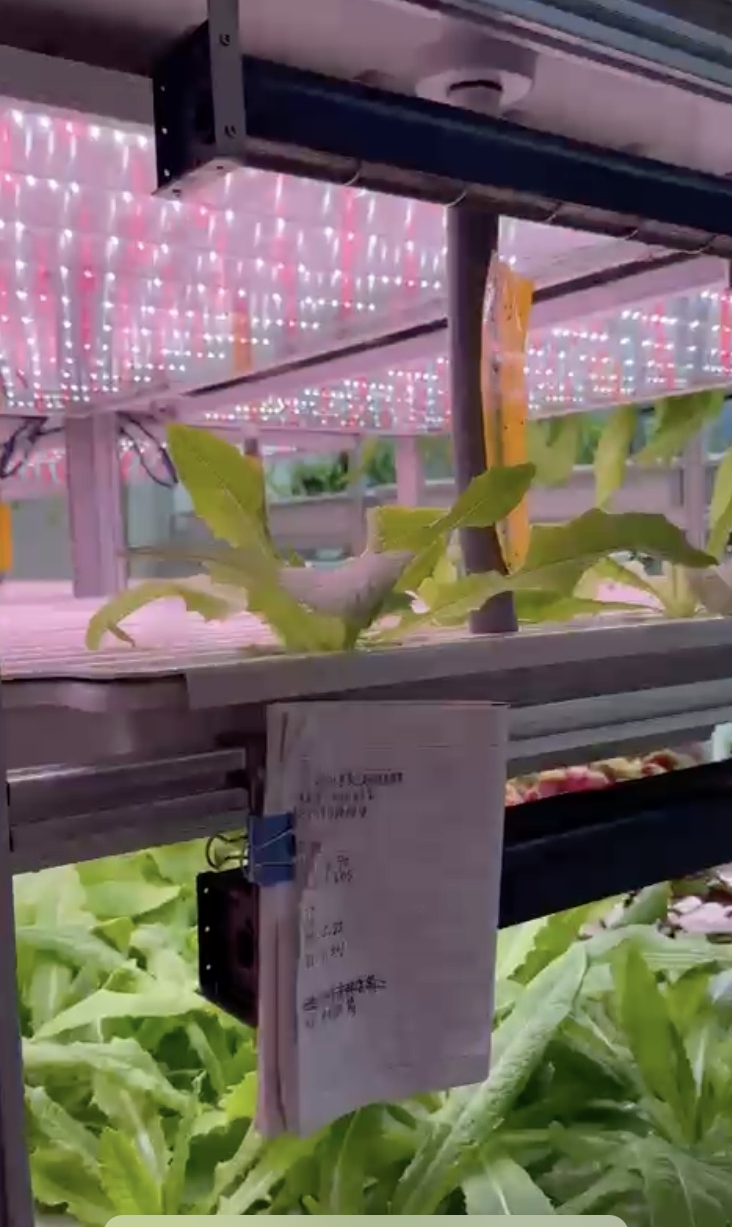
\includegraphics[height=13cm]{media/ekon2/image49}
        \caption*{}
    \end{subfigure}
    \begin{subfigure}[t]{0.45\textwidth}
        \centering
        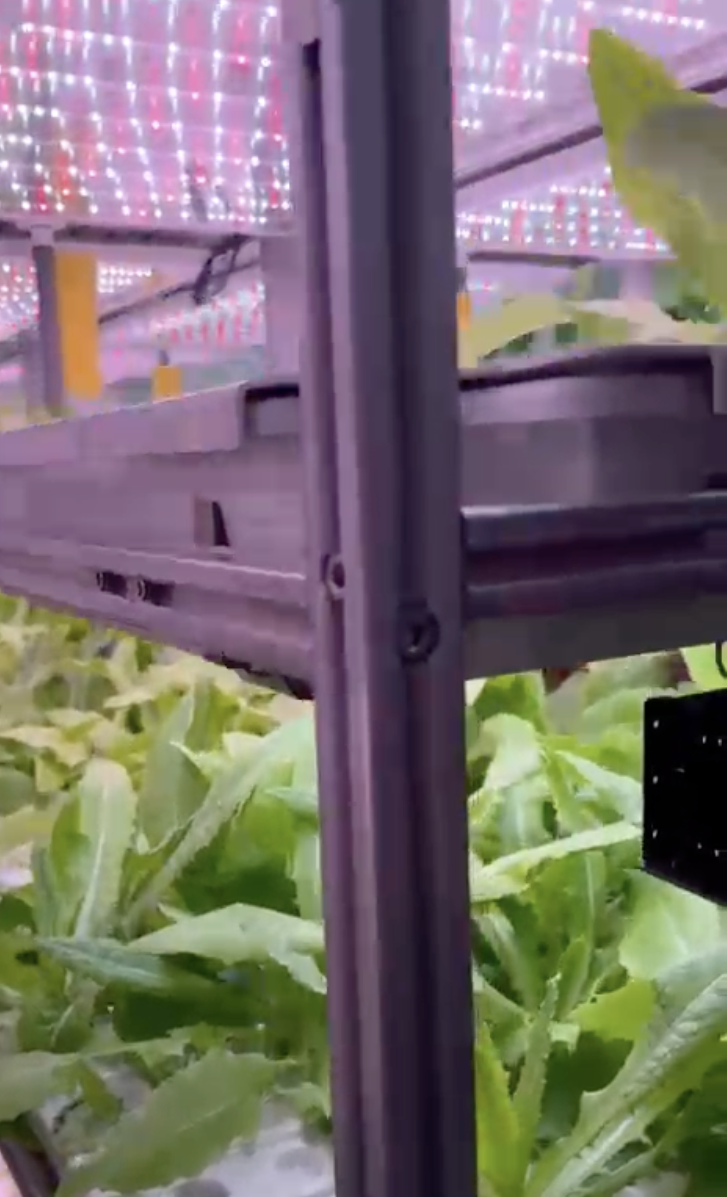
\includegraphics[height=13cm]{media/ekon2/image50}
        \caption*{}
    \end{subfigure}
    \caption*{Рис.4 - Специализированные экспериментальные установки}
    \caption*{\normalfont\emph{Примечание -- составлено авторами на основание данных проекта}}
\end{figure}

\begin{multicols}{2}
Следует отметить, что впервые в рамках данного проекта были разработаны
и использованы в качестве эксперимента управляемые светодиодные
прожекторы ABC1 и ABC2 отечественного производства для выращивания
томатов и салата.

Стоит отметить, что эффективность внедрения предлагаемых в исследование
технологий интегрированных систем вертикального фермерства раскрывается
посредством следующих аспектов:

- рост урожайности. Например, показатели урожайности вертикальных ферм
значительно превосходят традиционное сельское хозяйство. Например:
картофель: 150 т/га против 28 т/га; помидоры: 155 т/га (вертикально)
против 45 т/га (традиционно); перец: 133 т/га против 30 т/га. Стоит
отметить, что средний фактор увеличения урожайности: примерно около 2,5
раза, а с учетом укладки в вертикальном пространстве --- до 516\%
(таблица 1 статьи);

- снижение потребления ресурсов: водные ресурсы уменьшаются на 95\% по
сравнению с традиционным сельскии хозяйством, касательно удобрений
наблюдается экономия до 50\%; возможно полное исключение пестицидов,
гербицидов и фунгицидов;

- наблюдается уменьшение логистических издержек посредством размещения
вертикальных ферм в черте города, то есть отпадает необходимость в
транспортировки продукции на большие расстояния;

- соблюдение экологической устойчивости через минимальное воздействие на
окружающую среду: отсутствие загрязнения почв и водоемов, пропадает
необходимость в применение тяжёлой техники, применение возобновляемых
источников света такие как: специализированные LED-фитолампы (ABC1 и
ABC2), уменьшение выбросов CO₂ и прочих вредных веществ за счёт снижения
логистики и автономности вертикальных ферм;

- адаптивность и автономность, которая проявляется через систему,
которая полностью управляется дистанционно посредством компьютерных
технологий, применение искусственного интеллекта для оценки и анализа
данных, расчета урожайности, прогнозирования рисков и так далее;

- круглогодичное производство, которое проявляется через независимость
от климатических условий региона, также возможность круглогодичного
цикла выращивания, что особенно важно в городах с суровыми зимами
(например, Казахстан);

- перспективность для развития малого и среднего бизнеса, например,
создание «ферм под ключ» и разработка цифровых решений для управления,
привлекательность для инвесторов, большое разнообразие выращиваемой
продукции - до 250 культур.

Таким образом, внедрение технологий интегрированных вертикальных ферм
показывает значительную эффективность в аграрно-экономическом,
экологическом и социальном моментах жизни. Данные системы дают
возможность решать ключевые задачи продовольственной безопасности,
уменьшить затраты, увеличить урожайность, адаптировать к городским
условиям и климатическим изменениям. Именно приведенные примеры делают
рассматриваемые технологии вертикального фермерства перспективными для
стран с ограниченными ресурсами и быстрорастущим городским населением.

{\bfseries Выводы.} В целом, вертикальное фермерство является перспективным
подходом, который привлекает значительные инвестиции в сельское
хозяйство и экономику. На современном этапе развития разработка и
оптимизация вертикального фермерства направлена на улучшение
сельскохозяйственного производства в городских условиях. Вертикальное
фермерство изменит сельское хозяйство будущего, поскольку оно несет в
себе значительные преимущества: самое важное из них - снижение ущерба
окружающей среде и сохранение больших площадей для других целей.
Интегрированные системы вертикального фермерства также решают две
основные проблемы: сложность транспортировки сельскохозяйственной
продукции в города и обеспечение высокого качества продуктов питания с
помощью необходимых пестицидов и удобрений.

Стоит отметить, что сельскохозяйственная продукция
вертикально-интегрированных фермерских систем ни в чем не уступает
продуктам, производимым традиционным сельским хозяйством, - более того,
она превосходит их. Вертикальное фермерство имеет множество преимуществ,
включая высокую урожайность, возможность выращивать культуры круглый год
и потенциал для использования в городских районах. С развитием
технологий спрос на вертикальное земледелие растет, а рынок
увеличивается. Поскольку рынок растет в геометрической прогрессии, этот
сельскохозяйственный сектор становится выгодным для бизнеса, особенно в
густонаселенных городских районах.

\emph{{\bfseries Финансирование.}} \emph{Данное исследование было
реализовано при финансовой поддержке Комитета науки Министерства науки и
высшего образования Республики Казахстан в рамках ПЦФ ИРН: BR24992852 на
тему «Разработка интеллектуальных моделей и методов цифровой экосистемы
Smart City для устойчивого развития города и повышения качества уровни
жизни горожан».}
\end{multicols}

\begin{center}
{\bfseries Литература}
\end{center}

\begin{references}
1. Туртулова И.Р. Вертикальные фермы как основа для экологически
устойчивого АПК\textsc{/ В} сборнике: научные исследования студентов в
решение актуальных проблем АПК. Материалы всероссийской студенческой
научно-практической конференции. п. Молодежный. - 2022. -Т.2. - С.
89-95.

2. Libia I. Trejo-Téllez and Fernando C. Gómez-Merino. Nutrient Solutions
for Hydroponic Systems // Hydroponics - A Standard Methodology for Plant
Biological Researches.-2012.- P.1-22. DOI \\10.5772/37578

3. Груднева А.А. Вертикальное фермерство как интонационная технология
решения проблемы продовольственного снабжения крупных городов//Инновации
и инвестиции.- 2018. - № 9. - С.39-41.

4. Дмитриева А.С. Вертикальные фермы- новая тенденция в сельском
хозяйстве // Хроноэкономика. - 2019. - №~6~(19). - С.35-38.

5. Буторин С. Инновационно-ориентированная система управления аграрными
предприятиями // \\АПК: Экономика, управление. - 2016. - № 7.- С.40 -- 47.

6. Marczewska Magdalena, Sanaullah Ahmed, Tucci Christopher. Business
model configurations for suc\-cessful vertical farming// European journal
of innovation management.- 2025.-Vol.28( 4). - P.1555 - 1580 DOI
\href{http://dx.doi.org/10.1108/EJIM-01-2023-0017}{http://dx.doi.org}

7. Xiao Z., Lester G. E., Luo Y., Wang Q. Assessment of Vitamin and
Carotenoid Concentrations of Emerging Food Products: Edible
Microgreens// In Journal of Agricultural and Food Chemistry. American
Chemical Society (ACS).- 2012. -Vol.60(31). - P.7644-7651. DOI
\href{https://doi.org/10.1021/jf300459b}{10.1021/jf300459b}

8. Projected vertical farming market worldwide from 2022 to 2032 -
\href{https://www.statista.com/statistics/487666/projection-vertical-farming-market-worldwide/}{https://www.statista.com}
. Дата обращения: 14.12.2024.

9. Treadwell D., Hochmuth R., Landrum L., Laughlin W. Microgreens: A New
Specialty Crop// In EDIS. University of Florida George A Smathers
Libraries.- 2020. - Vol.2020(5). DOI 10.32473/edis-hs1164-2020

10. Guil-Guerrero J. L., Martínez-Guirado C., del Mar Rebolloso-Fuentes
M., Carrique-Pérez A. Nutrient composition and antioxidant activity of
10 pepper (Capsicum annuun) varieties// European Food Research and
Technology. -- 2006. - Vol.224(1). -- P.1-9
\href{https://doi.org/10.1007/s00217-006-0281-5}{DOI
10.1007/s00217-006-0281-5}

11. Clifford T., Howatson G., West D., Stevenson E. The Potential
Benefits of Red Beetroot Supplement\-ation in Health and Disease// MDPI
AG. In Nutrients. -- 2015. - Vol.7(4)- P.2801--2822.\\
\href{https://doi.org/10.3390/nu7042801}{DOI 10.3390/nu7042801}

12. Zheng W., Wang S. Y. Antioxidant Activity and Phenolic Compounds in
Selected Herbs// Journal of Agricultural and Food Chemistry. - 2001. -
Vol.49(11)11.- P.5165-5170 DOI 10.1021/jf010697n

13. Эскобар Х.П., Сандоваль А.А., Биензи П.М., Саласар Х.Д. Здания
вертикальных ферм в умных городах// Системные технологии. - 2020. -
№~1~(34). - С.73-76.

14. Илющенко Е.В. Глотова Н.И. Применение технологий искусственного
интеллекта в сельском хозяйстве // Перспективы внедрения инновационных
технологий в АПК: сборник статей//Российской (Национальной)
научно-практической конференции-Алтайский государственный аграрный
универ\-ситет, 2019.-С172-173.
\end{references}

\begin{center}
{\bfseries References}
\end{center}

\begin{references}
1. Turtulova I.R. Vertikal' nye fermy kak osnova dlja
jekologicheski ustojchivogo APK/ V sbornike: nauchnye issledovanija
studentov v reshenie aktual' nyh problem APK. Materialy
vserossijskoj studench\-eskoj nauchno-prakticheskoj konferencii. p.
Molodezhnyj. - 2022. -T.2. S.89-95. {[}In Russian{]}

2. Libia I. Trejo-Téllez and Fernando C. Gómez-Merino. Nutrient Solutions
for Hydroponic Systems // Hydroponics - A Standard Methodology for Plant
Biological Researches.-2012.- P.1-22. DOI \\10.5772/37578

3. Grudneva A.A. Vertikal' noe fermerstvo kak
intonacionnaja tehnologija reshenija problemy
prodovol' stvennogo snabzhenija krupnyh
gorodov//Innovacii i investicii.- 2018. - № 9. - S.39-41.

4. Dmitrieva A.S. Vertikal' nye fermy- novaja tendencija v
sel' skom hozjajstve//Hronojekonomika. - 2019. - № 6
(19). - S.35-38. {[}In Russian{]}

5. Butorin S. Innovacionno-orientirovannaja sistema upravlenija
agrarnymi predprijatijami// APK: \\Jekonomika, upravlenie. - 2016. - № 7.-
S.40 - 47. {[}In Russian{]}

6. Marczewska Magdalena, Sanaullah Ahmed, Tucci Christopher. Business
model configurations for suc\-cessful vertical farming// European journal
of innovation management.- 2025.-Vol.28( 4). - P.1555 - 1580 DOI
\href{http://dx.doi.org/10.1108/EJIM-01-2023-0017}{}

7. Xiao Z., Lester G. E., Luo Y., Wang Q. Assessment of Vitamin and
Carotenoid Concentrations of Emerging Food Products: Edible
Microgreens// In Journal of Agricultural and Food Chemistry. American
Chemical Society (ACS).- 2012. -Vol.60(31). - P.7644-7651. DOI
\href{https://doi.org/10.1021/jf300459b}{10.1021/jf300459b}

8. Projected vertical farming market worldwide from 2022 to 2032 -
\href{https://www.statista.com/statistics/487666/projection-vertical-farming-market-worldwide/}{https://www.statista.com}
. Дата обращения: 14.12.2024.

9. Treadwell D., Hochmuth R., Landrum L., Laughlin W. Microgreens: A New
Specialty Crop// In EDIS. University of Florida George A Smathers
Libraries.- 2020. - Vol.2020(5). DOI 10.32473/edis-hs1164-2020

10. Guil-Guerrero J. L., Martínez-Guirado C., del Mar Rebolloso-Fuentes
M., Carrique-Pérez A. Nutrient composition and antioxidant activity of
10 pepper (Capsicum annuun) varieties// European Food Research and
Technology. -- 2006. - Vol.224(1). -- P.1-9
\href{https://doi.org/10.1007/s00217-006-0281-5}{DOI
10.1007/s00217-006-0281-5}

11. Clifford T., Howatson G., West D., Stevenson E. The Potential
Benefits of Red Beetroot Supplement\-ation in Health and Disease// MDPI
AG. In Nutrients. -- 2015. - Vol.7(4)- P.2801--2822.
\href{https://doi.org/10.3390/nu7042801}{DOI \\10.3390/nu7042801}

12. Zheng W., Wang S. Y. Antioxidant Activity and Phenolic Compounds in
Selected Herbs// Journal of Agricultural and Food Chemistry. - 2001. -
Vol.49(11)11.- P.5165-5170 DOI 10.1021/jf010697

13. Escobar H.P., Sandoval A.A., Benzin P.M., Salazar H.D. Zdaniya
vertikal' nyh ferm v umnyh gorodah// Sistemnye
tekhnologii. - 2020. - № 1 (34). - Pp.73-76. {[}In Russian{]}

14. Ilyushenko E.V. Glotova N.I. Primenenie tekhnologij iskusstvennogo
intellekta v sel' skom hozyajstve // Perspektivy
vnedreniya innovacionnyh tekhnologij v APK: sbornik statej//Rossijskoj
(Nacional' noj) nauchno-prakticheskoj
konferencii-Altajskij gosudarstvennyj agrarnyj universitet,
2019. -S172-173. {[}In Russian{]}
\end{references}

\begin{authorinfo}
\emph{{\bfseries Сведения об авторах}}

Булхаирова Ж.С. - доктор PhD, ассоциированный профессор, Astana IT
University» LLP, Астана, Казахстан, е-mail: honeyzhu@mail.ru;

Шоман А.Е. - доктор PhD, ассоциированный профессор, Astana IT
University» LLP, Астана, Казахстан, е-mail: \\a.shoman@astanait.edu.kz;

Байдаков А.К. - к.э.н., ассоциированный профессор, Казахский
агротехнический исследовательский университет им. С.Сейфуллина, Астана,
Казахстан, e-mail: a\_baidakov@mail.ru

\emph{{\bfseries Information about the authors}}

Bulkhairova Zh.S. -- PhD, Associate Professor, Astana IT University LLP,
Astana, Kazakhstan, e-mail: honeyzhu@mail.ru;

Shoman A.E. - PhD, Associate Professor, Astana IT University LLP,
Astana, Kazakhstan, e-mail: a.shoman@astanait.edu.kz;

Baidakov A.K. - Candidate of Economic Sciences, Associate Professor,
S.Seifullin Kazakh Agrotechnical Research University, Astana,
Kazakhstan, e-mail: a\_baidakov@mail.ru
\end{authorinfo}
